\documentclass[a4paper,12pt]{article}
\usepackage{a4wide}
\usepackage{tikz}
\usetikzlibrary{calc}
\usepackage{hyperref}

\begin{document}
\pagestyle{empty}
\setlength{\parindent}{0em} 
\section*{ROM (Instruction Memory)}


Your task is to program the behavior of an entity called "ROM". This entity is declared in the attached file "ROM.vhdl" and has the following properties:
\begin{itemize}
\item Inputs: Clk and enable with type std\_logic; these are clock cycle and enable signals
\item Inputs: addr with type std\_logic\_vector; the address of instruction which is going to be read
\item Outputs: output with type std\_logic\_vector; this is the data (instruction) which is read 
\end{itemize}
\vspace{0.3cm}
\begin{center}
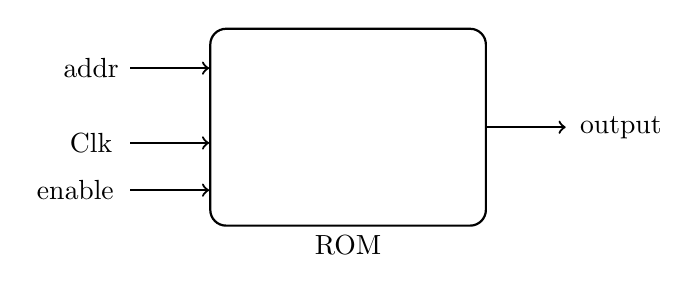
\begin{tikzpicture}
\draw node [draw,rectangle, minimum height=25mm, minimum width=35mm,rounded corners=2mm,thick](entity){};
\draw[->,thick] ($ (entity.west)-(10mm,-7.5mm)$) -- ($ (entity.west) - (0mm,-7.5mm)$);
\draw node at ($ (entity.west)-(15mm,-7.5mm)$){addr};
\draw[->,thick] ($ (entity.west)-(10mm,2mm)$) -- ($ (entity.west) - (0mm,2mm)$);
\draw node at ($ (entity.west)-(15mm,2mm)$){Clk};
\draw[->,thick] ($ (entity.west)-(10mm,8mm)$) -- ($ (entity.west) - (0mm,8mm)$);
\draw node at ($ (entity.west)-(17mm,8mm)$){enable};

\draw[->,thick] ($ (entity.east) + (0mm,0mm)$) -- ($ (entity.east) + (10mm,0mm)$);
\draw node at ($ (entity.east) + (17mm,0mm)$){output};



\draw node at ($ (entity) - (0,15mm)$){ROM};

\end{tikzpicture}
\end{center}

Do not change the file "ROM.vhdl".\\

The "ROM" entity shall behave according to the following ROM:\\

It has an input which is address, clock cycle and enable signals. The length of address is %%ADDRLENGTH bits, and the length of instruction is %%INSTRUCTIONLENGTH which is the same as the output. The ROM works on %%CLK of the clock cycle. \\

You need to write the VHDL code of ROM and fill it with the sample list of instructions as below. Write the instructions from address %%START to address %%STOP in the same sequence as they are written here. \\
Instructions:
\begin{center}
%%DATA\newline
\end{center}

The content of other locations in the ROM is zero.
\\

When the ROM is disabled the outputs are null and when it is enabled it reads the instruction which is in the input address and then outputs it. 

This behavior has to be programmed in the attached file "ROM\_beh.vhdl".\\

To turn in your solution, write an email to %%SUBMISSIONEMAIL with Subject "Result Task %%TASKNR" and attach your file "ROM\_beh.vhdl".

\vspace{0.7cm}

Good Luck and May the Force be with you.



\end{document}
\grid
\grid
\grid
\grid
